\documentclass[11pt,a4paper]{scrartcl}

\usepackage[ngerman,english]{babel}
\usepackage{graphicx}
\graphicspath{{pics/}}

\title{Hair Simulation with OpenCL}
\author{Etienne Gramlich \& Heiko Ettwein}


\begin{document}
\maketitle
\tableofcontents
\newpage
\pagenumbering{arabic}

\section{Introduction}

\subsection{Project Description}


\section{Implementation}

\subsection{Architecture}

\subsection{OpenCL}

\subsection{OpenGL}


\section{Hair Physics}
simple force model, no bounding boxes, small random differences of hair masses

\subsection{Force Model}
acceleration vectors, velocity, mass, linear combination of vectors

\subsubsection{Gravity}
gravitational force

\subsubsection{Elasticity}
link force \\ spring force

\begin{figure}[htbp]
\centering
\fbox{
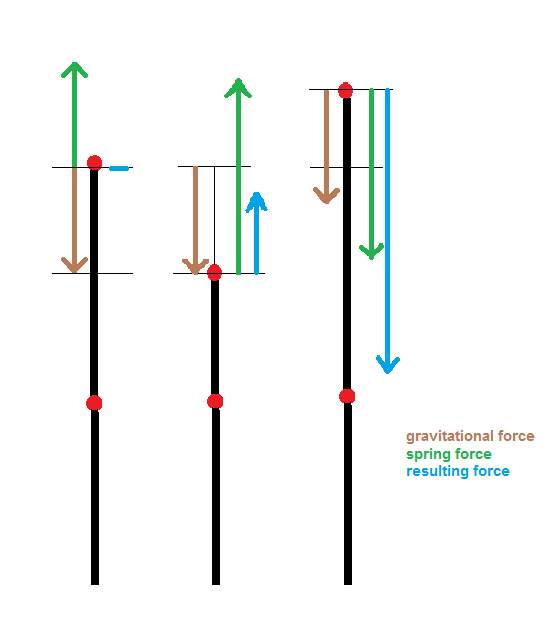
\includegraphics[width=1.0\textwidth]{SpringForce.png}
}
\caption{Spring force}
\end{figure}

\begin{figure}[htbp]
\centering
\fbox{
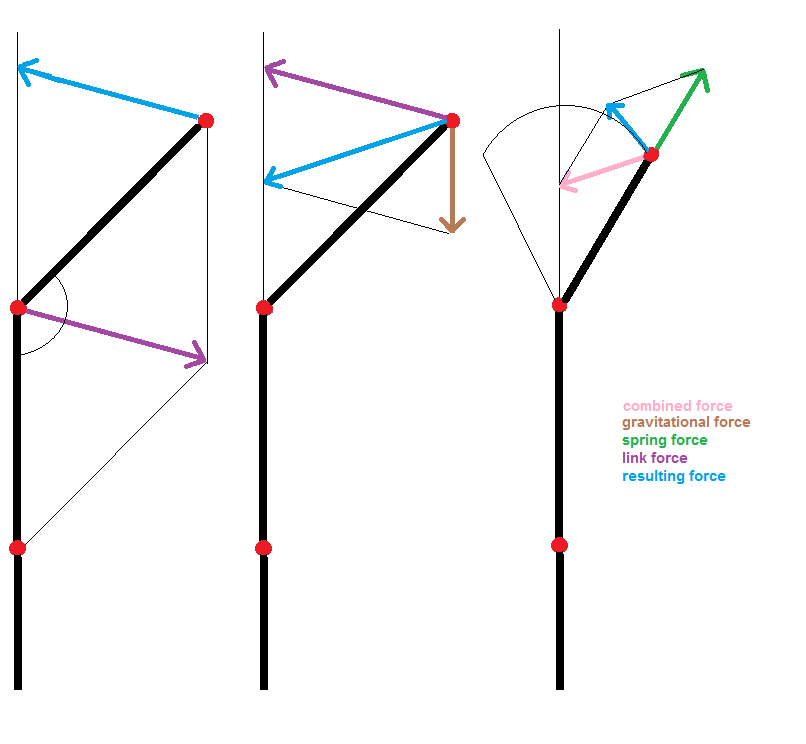
\includegraphics[width=1.0\textwidth]{CombinedForce.png}
}
\caption{Combination of all forces}
\end{figure}


\newpage
\subsubsection{Wind}
wind force \\ control direction and intensity (maximum force and interval)


\section{Conclusion}


\newpage
\section{Building}
The program can be built by importing the HairSimulation.sln in Visual Studio 2017 and then builing all sub-projects.

To run the program two files must be copied: The two shaders in \verb|HairSim\OpenCLProject1\Sample\shader| (fragment.glsl and vertex.glsl) must be places in the same diretory as the executable HairSim.exe. The OpenCL kernel SolvePositionsFromLinksKernel.cl must also be present, but should be copied from Visual Stuidio while building.

\end{document}